\section{ENCODE data} \label{encode-data-sect}
The Encyclopedia of DNA Elements (ENCODE) project \citep{Dunham2012} is an international collaboration of research groups with diverse backgrounds and expertise in production and analysis of NGS genomic data. \emph{Fig. \ref{seq-pic}} shows only some examples of the different platforms and techniques that are used from ENCODE to measure diverse biological components in order to interpret the human genome. That is, to discover functional elements in the genome, including genes, transcripts, transcriptional regulatory regions, chromatin structure and DNA methylation patterns.

\begin{figure}[!ht]
\begin{center}
 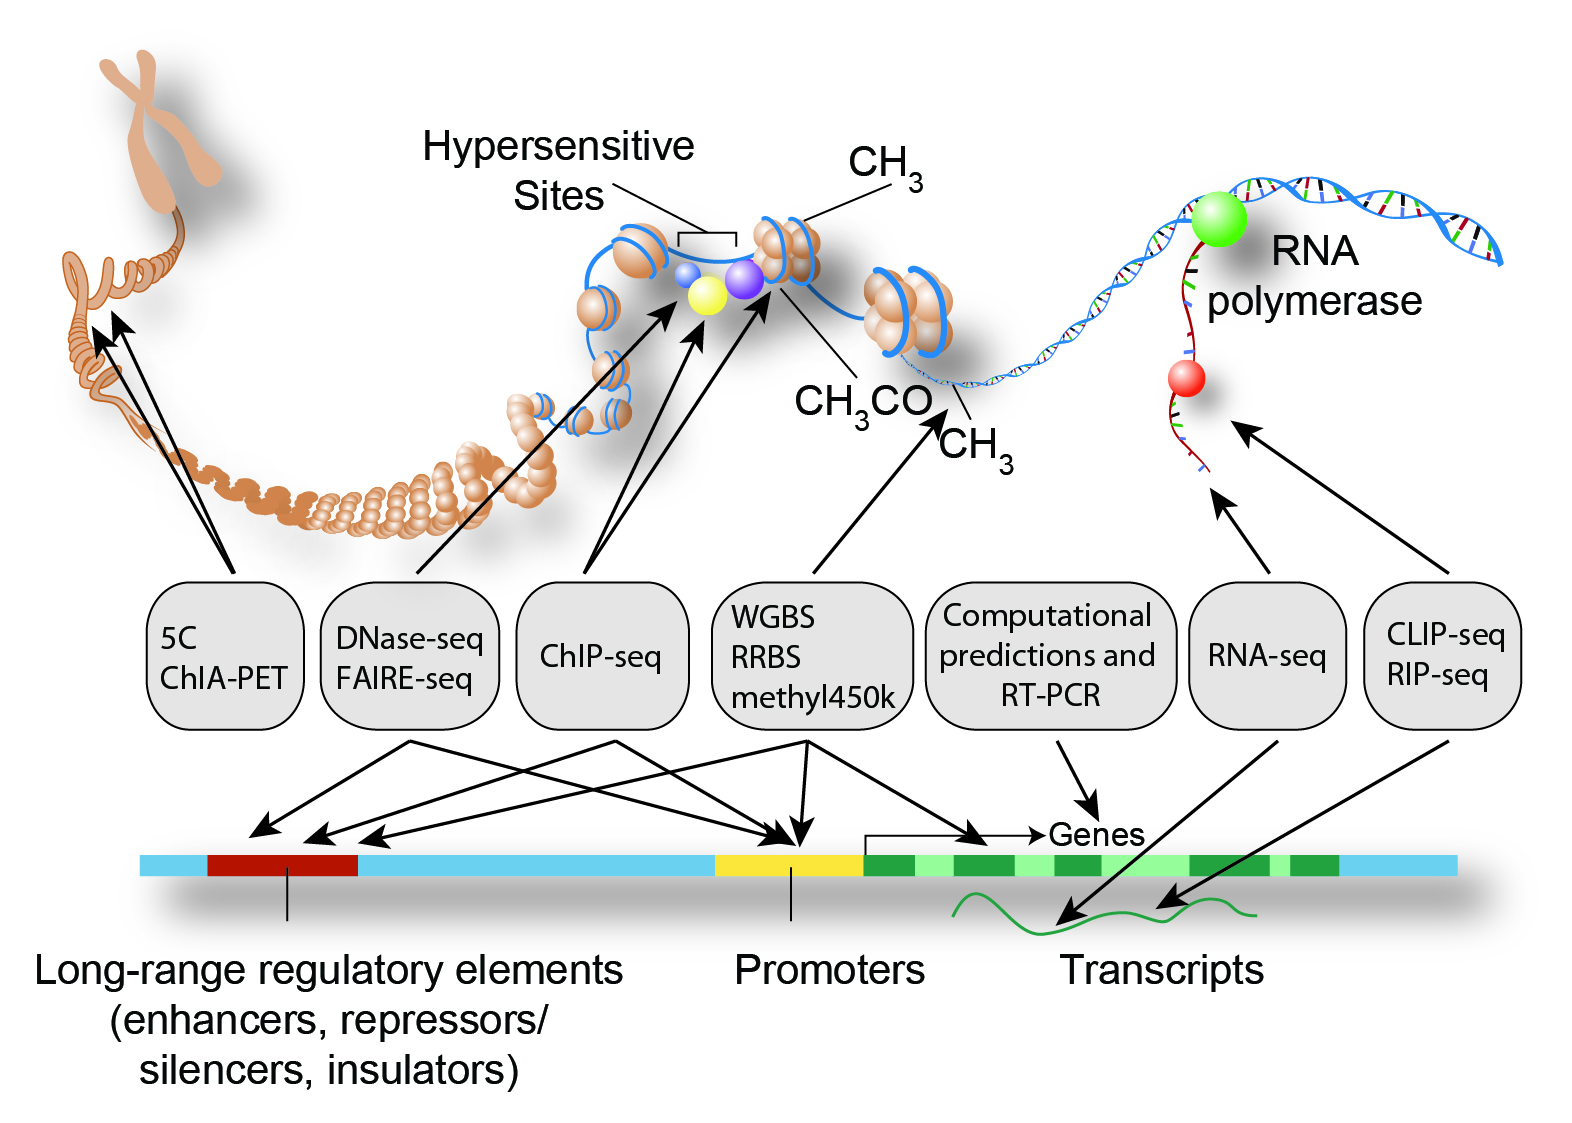
\includegraphics[scale = 0.25]{images/encode-seq.png}
\caption{\emph{Some of the XX-Seq techniques used from the ENCODE projet. Credits: Darryl Leja (NHGRI), Ian Dunham (EBI), Michael Pazin (NHGRI) \citep{Dunham2012}.}}
\label{seq-pic}
\end{center}
\end{figure} 

This project is mainly concentrated in modelling and analysing gene expression and DNA methylation data generated from NGS technology.